\documentclass{article}%
\usepackage[T1]{fontenc}%
\usepackage[utf8]{inputenc}%
\usepackage{lmodern}%
\usepackage{textcomp}%
\usepackage{lastpage}%
\usepackage[head=40pt,margin=0.5in,bottom=0.6in]{geometry}%
\usepackage{graphicx}%
%
\title{\textbf{Enfermedades bajo censura}}%
\author{Marielba Núñez | mnunez@el{-}nacional.com}%
\date{07/10/2018}%
%
\begin{document}%
\normalsize%
\maketitle%
\textbf{URL: }%
http://www.el{-}nacional.com/noticias/sociedad/enfermedades{-}bajo{-}censura\_254702\newline%
%
\textbf{Periodico: }%
EN, %
ID: %
254702, %
Seccion: %
Sociedad\newline%
%
\textbf{Palabras Claves: }%
Siete Días\newline%
%
\textbf{Derecho: }%
2.1%
, Otros Derechos: %
NO\_TIENE%
, Sub Derechos: %
2.1.1%
\newline%
%
\textbf{EP: }%
NO\newline%
\newline%
%
\textbf{\textit{La información epidemiológica ha sido cubierta por un manto de silencio, bajo el que han quedado soslayados algunos de los peores episodios que se han registrado en los últimos 11 años en materia de salud pública. Al menos 18 brotes o epidemias de malaria, dengue, influenza, parotiditis o sarampión han sido ocultados o se informaron a destiempo}}%
\newline%
\newline%
%
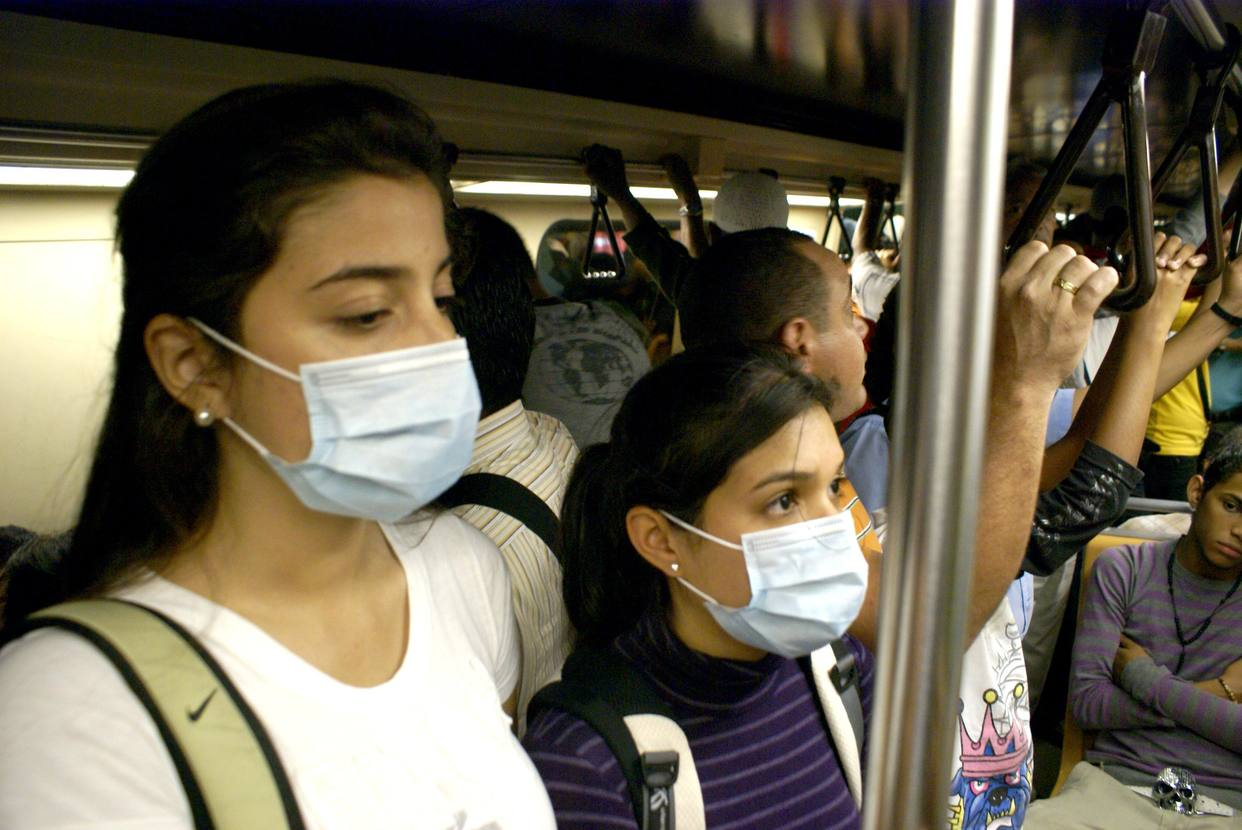
\includegraphics[width=300px]{159.jpg}%
\newline%
%
En Argentina, Brasil, Colombia, Ecuador y Perú se han registrado más de 1.600 casos de sarampión en 2018. En Brasil, además, ocurrieron 2.576 episodios de malaria en 2017. Todos ellos tuvieron en común que, como se ha establecido, habían sido importados de Venezuela o, en cuanto al sarampión, vinculados genéticamente con el virus que circula en el país.%
\newline%
%
La emigración venezolana ha llevado más allá de las fronteras las consecuencias del resquebrajamiento del sistema asistencial venezolano, al hacer evidente la actividad de enfermedades transmisibles que se daban por controladas en la región. La emergencia, si alguien se atiene a lo que señala un documento de la Organización Panamericana de la Salud, discutido hace poco en el consejo directivo de ese organismo, parece haber aparecido repentinamente: “Se han registrado brotes de difteria, sarampión y malaria que se han propagado con rapidez, afectando a muchos de los 23 estados del país y el Distrito Capital al mismo tiempo”, indica el texto que describe la crisis, bautizado con el rebuscado título de “Respuesta de la OPS para mantener una agenda eficaz de cooperación técnica en Venezuela y en los Estados miembros vecinos”.%
\newline%
%
La médica Marianella Herrera, presidenta del Observatorio Venezolano de~la Salud, señala en cambio que la emergencia humanitaria venezolana ha sido de instalación lenta y progresiva, pese a que~la OPS, así como otros organismos internacionales, parecen sorprenderse ahora por la magnitud del deterioro sanitario, que se expresa en cifras como los 1.217 casos y 168 muertes causadas por la difteria en los últimos 3 años; los 4.272 episodios de sarampión contabilizados desde 2017 o los 406.289 casos de malaria registrados solo el año pasado.%
\newline%
%
Los datos se conocen porque los difunde la propia OPS, pues no hay una fuente oficial venezolana que los dé a conocer. “Tal pareciera que los silencios epidemiológicos impuestos por las autoridades venezolanas cumplen el papel de ocultar la información para que no se sepa la verdad que permita tomar las medidas necesarias cuando hay un problema público de salud”, apunta Herrera.%
\newline%
%
El último boletín epidemiológico difundido oficialmente por el Ministerio de Salud corresponde a la semana final de 2016, y su publicación, en febrero de 2017, le costó el cargo poco después a la entonces ministra de Salud, Antonieta Caporale. El documento había visto la luz luego de más de 15 meses de silencio sobre las epidemias del país y tenía datos que ya movían al escándalo: la mortalidad infantil había aumentado 30\% con respecto a 2015, pues habían fallecido 11.466 niños menores de un año. Otro dato dramático en el boletín era que la mortalidad materna se había incrementado 66\%, pues en el mismo período fallecieron 756 embarazadas. Ese fue el último informe de su tipo del que se tiene noticia, lo cual significa que van 19 meses de silencio, en medio de la agudización de la crisis humanitaria incubada por la escasez de alimentos y medicinas.%
\newline%
%
Amenazas reiteradas.~La publicación del boletín epidemiológico había sido una tarea cumplida fielmente por el Ministerio de Salud desde 1938, por iniciativa del recordado~sanitarista~Darío Curiel Sánchez. Fue una idea pionera, reconocida internacionalmente, que enorgullecía a los médicos venezolanos, pero a mediados de 2007, mientras estaba al frente del ministerio Jesús Mantilla, comenzó a interrumpirse la difusión de ese instrumento, recuerda José Félix Oletta, ex ministro de Sanidad y Asistencia Social y miembro de la red Defendamos la Epidemiología Nacional, una de las organizaciones que ha asumido la tarea de constituir un frente paralelo para tratar de llenar el vacío de información.%
\newline%
%
“Es una política de Estado que corresponde a una visión autoritaria: pretenden tener el monopolio de la información, hasta de los datos epidemiológicos, pues quien maneja la información tiene el poder. No quieren someterse a ninguna contraloría social ni institucional, ni quieren ser cuestionados por el manejo de los recursos o por las fallas en los planes de prevención de enfermedades. Quieren ocultar su fracaso detrás de la hegemonía comunicacional”, señala Oletta.%
\newline%
%
El boletín epidemiológico, que se daba a conocer semanalmente, contenía información acerca de 72 enfermedades de notificación obligatoria en el país. El detallado seguimiento realizado por Oletta desde que comenzaron las interrupciones de ese documento desde hace 11 años, permite advertir que al menos 18 eventos epidémicos fueron ocultados o se informó tardíamente de ellos debido a la desaparición del documento. Uno de esos episodios fue la epidemia de fiebre chikungunya en 2014. Pese a que la enfermedad se detectó en el país en junio de ese año, pasaron 4 meses antes de que el Ministerio de Salud diera la orden de que se notificara obligatoriamente. Algo similar ocurrió con la difteria, enfermedad que reapareció en el país luego de 24 años sin que se presentaran casos, en abril de 2016, pero hubo reconocimiento oficial varios meses después, cuando se reanudó la publicación del boletín epidemiológico, a principios de 2017. Solo entonces la opinión pública pudo saber con certeza que habían ocurrido 324 casos durante ese año.%
\newline%
%
Situaciones similares se han sucedido con eventos como las epidemias de sarampión, malaria, parotiditis y zika, entre otras. La política oficial parece resumirse en declaraciones en 2013 de la ministra de Salud Isabel Iturria, quien cuando fue interrogada sobre el impacto de la gripe AH1N1, manifestó: “Yo no voy a decir los números”. O en las que expresó el ex ministro Henry Ventura en 2014, cuando advirtió que el boletín epidemiológico no iba a salir “más nunca”.%
\newline%
%
Otra recordada frase, que resume lo que ha sido la posición gubernamental, fue proferida por Luis Montiel, director de Epidemiología del Ministerio de Salud, en 2008: “Si empiezan a utilizar el boletín epidemiológico para desestabilizar, para el golpismo o para el terrorismo, no podemos permitir que con nuestro propio instrumento que estamos empleando para la toma de decisiones y la mejora de la salud del pueblo, vengan los medios de comunicación a hacer oposición y hagan terrorismo mediático, y le creen un problema de salud mental a la población venezolana”.%
\newline%
%
La negativa oficial a difundir información ha sido refrendada por otros poderes públicos. Basta recordar cuando, en 2010, la Sala Constitucional del Tribunal Supremo de Justicia declaró inadmisible el recurso de amparo interpuesto por las ONG Espacio Público y Provea para que se divulgara la información epidemiológica.%
\newline%
%
En el actual Ministerio de Salud la opacidad persiste. La página web, suspendida en 2017, fue reactivada hace poco pero no contiene información actualizada. El más reciente anuario de mortalidad corresponde a 2014 y los últimos indicadores epidemiológicos a 2008. Los boletines epidemiológicos, tal como se conocían, no están disponibles. En la Dirección de Vigilancia Epidemiológica, en el piso 7 del Ministerio de Salud, explican que “hay información que se publica y otra no; la página web del ministerio está en reestructuración, pero hasta nuevo aviso no va a salir una actualizada con toda la información”. Se intentó conversar con el director de Epidemiología, José Manuel García, para que suministrara una explicación más detallada, pero no respondió la solicitud.%
\newline%
%
Opacidad generalizada.~Los boletines epidemiológicos y los anuarios de morbilidad y mortalidad forman parte de una larga lista de documentos oficiales llamados a dar cuenta del estado de salud de la población, que han sido vedados a la opinión pública. Oletta apunta que también desapareció el boletín integral de salud ambiental, que era publicado por el Instituto de Altos Estudios de Salud Pública Arnoldo Gabaldón, y que contenía datos sobre las endemias rurales, entre ellas chagas, dengue, malaria y parasitosis. "Toda esa información, de manera sistemática, fue eliminada y restringida en forma arbitraria”, indica.%
\newline%
%
A ello se añade la ausencia de las hojas de balance de alimentos del Instituto Nacional de Nutrición, documento técnico que permite establecer cuál es la comida disponible en el territorio y traducirla en la cantidad de nutrientes que significa para la población. En la página web del INN puede advertirse que el último documento de ese tipo que está disponible data de 2014.%
\newline%
%
La especialista en infectología Ana Carvajal, también miembro de la red Defendamos la Epidemiología Nacional, considera que la decisión oficial de ocultar la información sobre epidemias y enfermedades transmisibles pretende ocultar el fracaso de las políticas de salud en Venezuela. “Ya perdimos, por ejemplo, la certificación de la eliminación del sarampión porque tenemos más de un año con casos. También hay un incremento de tuberculosis y de VIH. Sobre este último virus, sin duda se han incrementado las cifras de mortalidad porque el año pasado prácticamente no hubo tratamiento antirretroviral y el suministro comenzó a reactivarse hace apenas dos meses. Personas que estaban más o menos estables tuvieron que interrumpir la terapia, lo cual las deja a merced de infecciones oportunistas”, dice. “El abandono del tratamiento ha sido por desabastecimiento, que también causa ansiedad y angustia”.%
\newline%
%
Carvajal describe el Ministerio de Salud como una verdadera “caja negra”, que maneja la información a discreción. Sin embargo, esa cortina de hierro tiene algunas filtraciones que son las que han permitido a los activistas y a los expertos tener acceso a algunos de los datos que les permiten medir las condiciones de salud de la población, muchas veces gracias a publicaciones internacionales. Fue el caso de la difteria, pues en 2017 se conoció la enfermedad a través de los boletines epidemiológicos publicados en Cuba, recuerda Oletta.%
\newline%
%
Los documentos de la OPS se están convirtiendo también en otra vía para tener acceso a la información, aunque sea tardíamente. “La paradoja es que se enteran primero en Ginebra o en Washington de lo que está ocurriendo aquí”, se queja el ex ministro. El texto discutido en la reunión del consejo directivo del organismo internacional que finalizó el 27 de septiembre es un ejemplo de ello, pues tiene los datos actualizados sobre varias de las epidemias activas en el país y su impacto regional. También contiene una serie de recomendaciones para el gobierno venezolano, entre ellas una que tiene que ver con la difusión de los datos. El país debe “mejorar las funciones esenciales de salud pública, incluida la vigilancia y la disponibilidad de información de salud en el contexto del Reglamento Sanitario Internacional”.%
\newline%
%
Se trata sin duda de un punto importante para el organismo y la seguridad de la región. Una situación irregular, que habla de hasta qué punto han fallado los canales de comunicación de la información que el ministerio debe ofrecer a organismos internacionales fue el caso de parálisis flácida, vinculada con el virus de la polio, reportado por la OPS en junio de 2018. Pese a que los análisis concluyeron luego que la alarma inicial por la posible reaparición del virus debía ser descartada, fue significativo que el Ministerio de Salud incumplió con los procedimientos pues no hizo la notificación del caso a la Organización Mundial de la Salud en las 24 horas reglamentarias. “Cuando hay una situación de esa naturaleza no se debe dejar pasar más de 48 horas, y tardaron en dar la información no menos de 2 meses. Si los datos no hubieran llegado a los organismos internacionales por vías extraoficiales, no hubiera pasado absolutamente nada”, señala Oletta. El experto, sin embargo, expresa dudas acerca de cómo se manipuló la muestra que fue enviada a los laboratorios internacionales.%
\newline%
%
Carvajal añade que otra ausencia importante de información tiene que ver con el funcionamiento actual del Instituto Nacional de Higiene Rafael Rangel, organismo encargado de analizar las muestras biológicas que envían los centros de salud del país, resultados necesarios para dar un diagnóstico. “Muchas veces es información que se produce de forma extemporánea y cuesta mucho que los médicos la obtengan”.%
\newline%
%
Oletta puntualiza en qué se traduce la ausencia de datos: “Cuesta vida, cuesta sufrimiento. Solo con información puedes actuar con anticipación, y no cuando ya la curva de las epidemias ha avanzado. En nuestro caso, han pasado 2 años y seguimos con casos de difteria, tenemos 15 meses con sarampión. Hemos exportado casos y nos hemos convertido en un problema regional. La información es garantía de una sociedad sana”.%
\newline%
%
\end{document}